\chapter{الدفاعات المناعية}\label{ch:g9:immune-defenses}

الأبواب ممسكة
(\cref{prop:g9:microbes-and-infection:doors}) --- ومع
ذلك يهبط غاز أحيانًا: \omterm{def:g9:microbes-and-infection:sorted}{بكتيريا} الشظية تتضاعف في النسيج
الدافئ، \omterm{def:g9:microbes-and-infection:sorted}{والفيروس} يطبع سلفًا في \omterm{def:g5:first-look-at-cells:cell}{خلايا} المسالك الهوائية.
وما يجري بعد ذلك هو ثالث أجهزة الجسم الكبرى بعد \omterm{def:g5:brain-in-command:system}{الأعصاب}
\omterm{def:g8:hormonal-communication:glands}{والهرمونات}: الدفاعات المناعية --- جيش قائم، وفيلق
اختصاصيين ذو ذاكرة، وحيلة \omterm{prop:g9:immune-defenses:vaccination}{التلقيح} التي تدربه سلفًا.

\section{الاستجابة السريعة: الالتهاب}

\begin{definition}[الجيش القائم]\label{def:g9:immune-defenses:standing}
تجوب \omterm{prop:g4:journey-of-food:absorb}{الدم} والأنسجة الكريات البيضاء\index{كرية بيضاء} ---
جنود الجهاز المناعي، تصنع في نقي \omterm{def:g3:bones-and-muscles:skeleton}{العظم}، وتركب شبكة
\cref{prop:g4:heart-and-blood:carries}. وأول المستجيبين
هي \emph{البالعات}: \omterm{def:g5:first-look-at-cells:cell}{خلايا} تسيل حول الدخيل فتهضمه (فقد
أجرت الكتلة السائلة في
\cref{ex:g6:cell-unit-of-life:drop} المناورة نفسها التي
يجريها صياد حر --- والجسم يوظف الحيلة القديمة دفاعًا).
\end{definition}

\begin{proposition}[الالتهاب، مقروءًا كما ينبغي]\label{prop:g9:immune-defenses:inflammation}
ما يعقب الشظية --- احمرار، ودفء، وتورم، وخفقان --- ليس
انتصار \omterm{def:g9:microbes-and-infection:stages}{العدوى} بل وصول الدفاع. فإشارات إنذار من النسيج
المتضرر توسع \omterm{def:g4:heart-and-blood:vessels}{الأوعية} الموضعية (إعادة التوجيه في
\cref{prop:g7:organs-at-work:supply}، وقد استدعيت): دم
دافئ أكثر، وجدران تجعل نافذة، وبالعات تنسل من الشعيرات
وتزحف إلى الموضع، تأكل \omterm{def:g9:microbes-and-infection:sorted}{البكتيريا} في طريقها. والقيح حصيلة
الميدان --- بالعات مستهلكة، وغزاة موتى، وحطام. وأكثر
الهبوطات تنتهي هنا، في أيام، من غير أن يلحظها أحد.
\end{proposition}
\admitted

\begin{example}[قراءة جرح يلتئم]\label{ex:g9:immune-defenses:cut}
اليوم الأول: هالة حمراء دافئة موجعة --- \omterm{def:g4:heart-and-blood:vessels}{الأوعية} واسعة،
والجنود يصلون. واليوم الثاني: قليل من القيح --- الحصيلة.
واليوم الرابع: الهالة تخبو، والقشرة جافة --- فقد خسر
التضاعف السباق أمام البلعمة، وإعادة بناء \omterm{def:g1:the-five-senses:sense}{الجلد}
(\cref{prop:g5:first-look-at-cells:growth}) تغلق الباب
خلف الحرب. حملة كاملة، خيضت وربحت دون مقياس القلق.
\end{example}

\section{الاختصاصيون: التعرف والذاكرة}

\begin{proposition}[الاستجابة النوعية]\label{prop:g9:immune-defenses:specific}
حين تسبق الاستجابة السريعة، ينزل فيلق الاختصاصيين
الميدان --- أبطأ، وأدق:
\begin{itemize}
  \item كل غاز يحمل علامات سطحية --- هي
        \emph{مستضداته}\index{مستضد} --- أشكال جزيئية
        يقرؤها الاختصاصيون غريبة (وعلامات الذات في
        \cref{ex:g9:unique-individuals:medicine} هي
        القراءة نفسها، مصوَّبة إلى الداخل)؛
  \item ومن بين \omterm{def:g9:immune-defenses:standing}{الكريات البيضاء} الاختصاصية، قليل يحمل
        مستقبلات تلائم \emph{هذا} \omterm{prop:g9:immune-defenses:specific}{المستضد}؛ فالتماس
        ينتقيها، فتتضاعف إلى جيش مستنسخ (منطق الانتقاء،
        مجرى داخل الجسم في أيام)؛
  \item وسلاحها: \emph{الأجسام المضادة}\index{جسم مضاد}
        --- جزيئات ملائمة تصب في \omterm{prop:g4:journey-of-food:absorb}{الدم} فتثبّت الغازي
        وتكتّله للبالعات --- واختصاصيون قتلة يدمرون
        \omterm{def:g5:first-look-at-cells:cell}{خلايا} الجسم المخطوفة نفسها، وهي الطريقة الوحيدة
        لإيقاف مطابع \omterm{def:g9:microbes-and-infection:sorted}{الفيروس}
        (\cref{ex:g9:microbes-and-infection:contrast})؛
  \item وكلفة المعركة جزء من المرض: الحمى (جسم يجري
        ساخنًا عن قصد --- فكثير من \omterm{prop:g9:microbes-and-infection:mostly}{الممرضات} تتضاعف أسوأ
        في الدفء)، والأوجاع، و\emph{العقد اللمفية}
        المتورمة --- ثكنات الاختصاصيين، مزدحمة في زمن
        الحرب.
\end{itemize}
\end{proposition}
\admitted

\begin{definition}[الذاكرة المناعية]\label{def:g9:immune-defenses:memory}
بعد النصر، يتنحى جزء من الجيش المستنسخ ليصير \emph{خلايا
ذاكرة}\index{خلية ذاكرة}: اختصاصيين طوال العمر يحملون
وصف \omterm{prop:g9:immune-defenses:specific}{المستضد}. وهبوط ثان للغازي \emph{نفسه} يلقى فيلقًا
مهيأً --- استجابة في ساعات، والغازي يزال قبل الأعراض:
فأنت \emph{منيع}\index{مناعة}. حصبة واحدة، لا اثنتان؛
وسلالة الشتاء الماضي عاجزة عن إشعال فاشية هذه السنة
(\cref{pb:g9:microbes-and-infection:1}). والذاكرة هي سبب
أن الزكام نفسه لا يبدو أنه يأتي مرتين --- وسبب أن الزكام
يظل يأتي: ففيروساته تطفر سريعًا
(\cref{prop:g9:genes-and-dna:explains}) إلى أوصاف لا
تحملها الذاكرة.
\end{definition}

\section{تدريب الدفاع: التلقيح}

\begin{proposition}[التلقيح]\label{prop:g9:immune-defenses:vaccination}
\emph{التلقيح}\index{تلقيح} ذاكرة مناعية تنشأ من غير
مرض: تعرض على الاختصاصيين \emph{وصف} الغازي ---
\omterm{def:g6:producing-our-food:fermentation}{ميكروبات} مقتولة أو موهنة، أو شظايا غير ضارة تحمل
\omterm{prop:g9:immune-defenses:specific}{المستضد} --- فيجري برنامج الانتقاء والذاكرة كله، ناقصًا
الخطر. ثم يلقى الفيلق المدرَّب الممرض الحقيقي، إن لقيه
يومًا، هبوطًا ثانيًا. ونتيجتان تحملان ثقل الصحة العامة:
\begin{enumerate}
  \item الملقَّحون محميون قبل المعركة الأولى --- وهو
        حاسم في أمراض قد تقتل معركتها الأولى أو تشوّه؛
  \item وجيران ملقَّحون بعدد كاف يجوّعون الفاشية من
        مضيفين قابلين للالتقاط (خمود
        \cref{pb:g9:microbes-and-infection:1}): فالحماية
        تتجمع --- والدرع يغطي من هم أصغر أو أمرض من أن
        يدرَّبوا بأنفسهم.
\end{enumerate}
\end{proposition}
\admitted

\begin{example}[من مقامرة جدري البقر إلى الاستئصال]\label{ex:g9:immune-defenses:history}
تمتد الحكاية من مقامرة جينر سنة 1796 --- إذ كانت حالبات
البقر يصبن بجدري البقر الخفيف ولا يصبن بالجدري قط؛
فتلقيح بجدري البقر يدرّب ضد القاتل --- مرورًا بلقاحات
باستور المتعمدة \omterm{def:g6:producing-our-food:fermentation}{بميكروبات} موهنة (صاحب
\cref{ex:g9:microbes-and-infection:history}، يتم
نظريته)، إلى كشوف القرن العشرين: الجدري، بلاء البشرية
القديم، \emph{مستأصلًا} --- \omterm{def:g9:microbes-and-infection:sorted}{والفيروس} \omterm{prop:g5:biodiversity:loss}{منقرض} في البرية منذ
أواخر سبعينيات القرن الماضي --- وشلل الأطفال مدفوعًا إلى
آخر زوايا الخريطة. فالذاكرة المدرَّبة، مجمَّعة، هي
السلاح الوحيد الذي أباد مرضًا بشريًا قط.
\end{example}

\begin{omfigure}
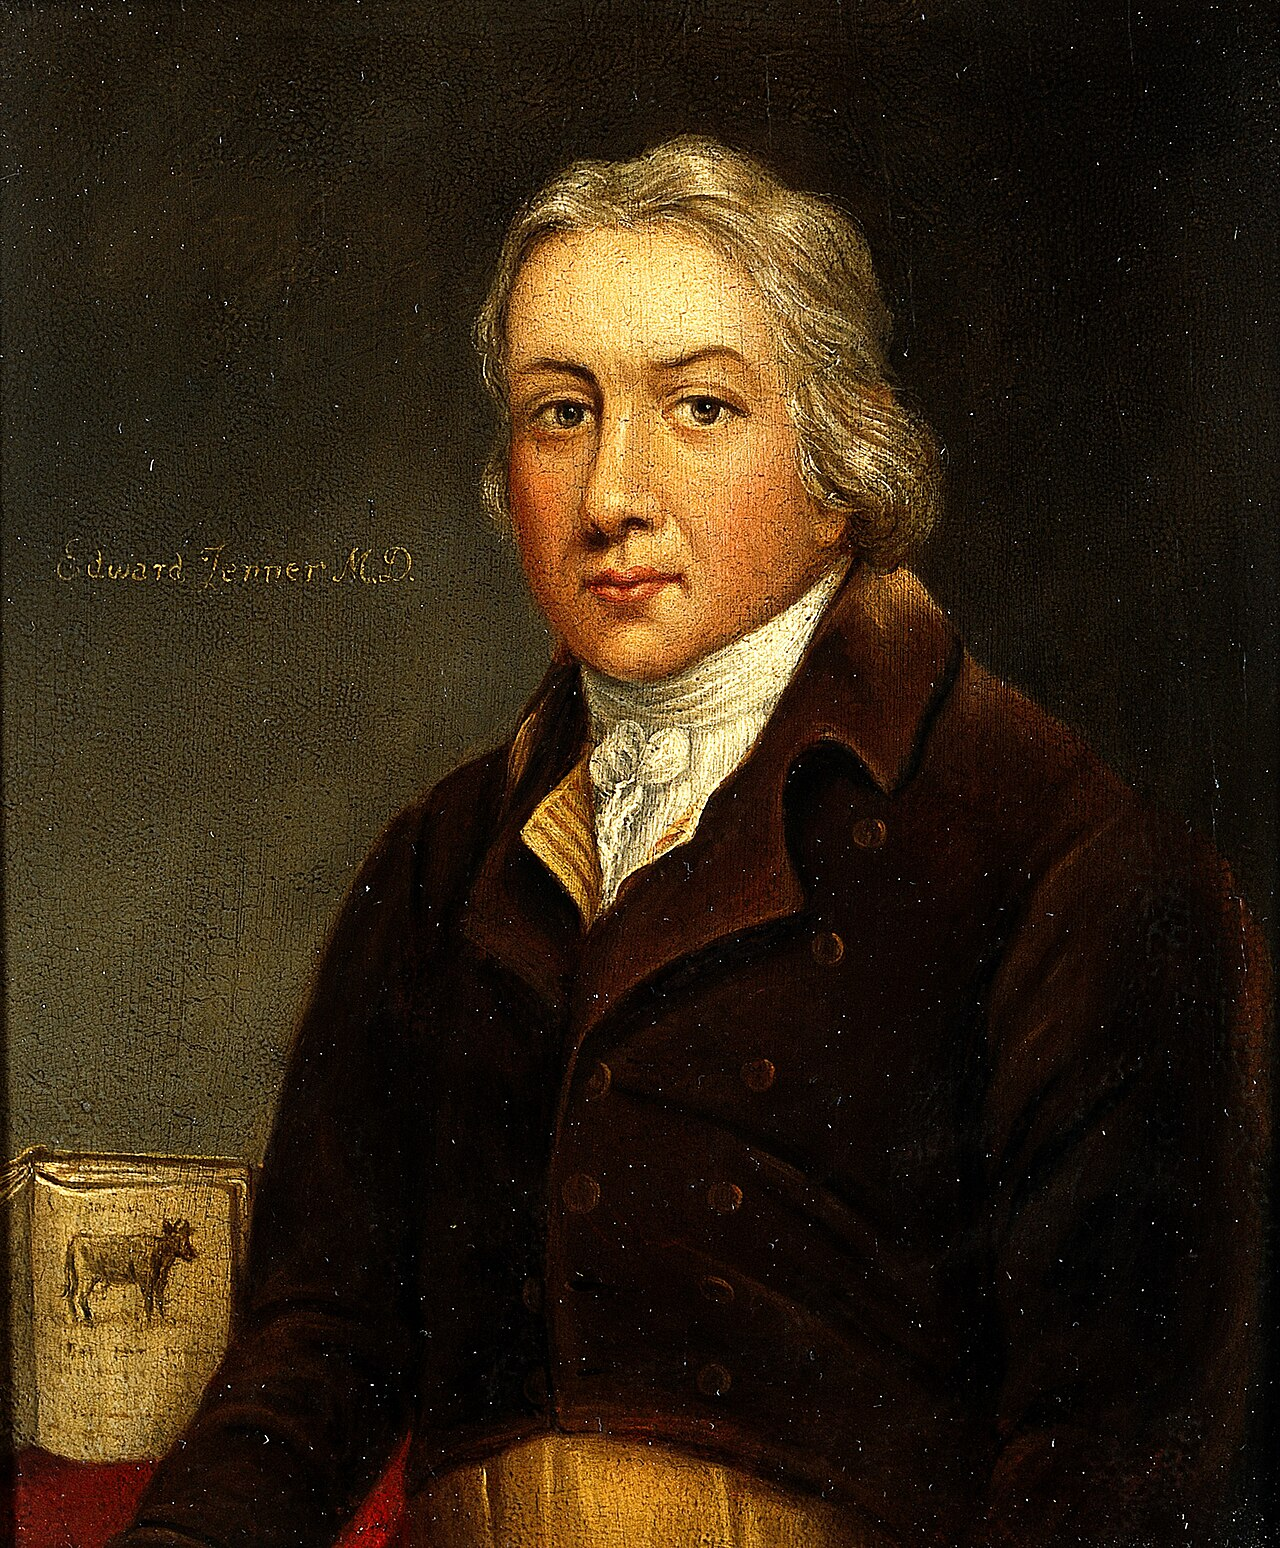
\includegraphics[width=0.46\linewidth]{images/book1/jenner.jpg}

{\small إدوارد جينر، صاحب مقامرة جدري البقر سنة 1796
التي صارت \omterm{prop:g9:immune-defenses:vaccination}{التلقيح}. تصوير زيتي، مجموعة Wellcome Collection،
CC~BY~4.0.}
\end{omfigure}

\begin{method}[قراءة أي حدث مناعي]\label{met:g9:immune-defenses:read}
في أي \omterm{def:g9:microbes-and-infection:stages}{عدوى}، أو تعاف، أو لقاح، أو نتيجة تحليل:
\begin{enumerate}
  \item حدد مرحلة اللقاء: أهبوط أول أم ثان؟ (فالذاكرة
        تغير كل شيء)؛
  \item وسمّ المستجيبين: استجابة البالعات السريعة، أم
        جيش الاختصاصيين المستنسخ، أم الذاكرة القائمة؛
  \item واقرأ العلامات كما ينبغي: الالتهاب والحمى دفاعًا
        في عمله، والعقد المتورمة ثكنات؛
  \item وفي اللقاح: عيّن الوصف المعروض، وحماية من تتجمع.
\end{enumerate}
\end{method}

\section{تمارين}

\begin{exercise}[$\star$]\label{exo:g9:immune-defenses:1}
من الجيش القائم ومن أول المستجيبين، وأين يصنعان؟
\end{exercise}

\begin{exercise}[$\star$]\label{exo:g9:immune-defenses:2}
ترجم علامات الشظية الأربع إلى أحداث دفاعية.
\end{exercise}

\begin{exercise}[$\star$]\label{exo:g9:immune-defenses:3}
ما \omterm{prop:g9:immune-defenses:specific}{المستضد}، وما \omterm{prop:g9:immune-defenses:specific}{الجسم المضاد}، وما الصلة بينهما؟
\end{exercise}

\begin{exercise}[$\star$]\label{exo:g9:immune-defenses:4}
لماذا وجب على الاختصاصيين القتلة أن يدمروا \omterm{def:g5:first-look-at-cells:cell}{خلايا} الجسم
نفسها في \omterm{def:g9:microbes-and-infection:stages}{عدوى} فيروسية؟
\end{exercise}

\begin{exercise}[$\star$]\label{exo:g9:immune-defenses:5}
ما \omterm{def:g9:immune-defenses:memory}{خلية الذاكرة}، وماذا يلقى الهبوط الثاني؟
\end{exercise}

\begin{exercise}[$\star$]\label{exo:g9:immune-defenses:6}
عرّف \omterm{prop:g9:immune-defenses:vaccination}{التلقيح} في جملة واحدة مبنية من ``وصف'' و``ذاكرة''.
\end{exercise}

\begin{exercise}[$\star\star$]\label{exo:g9:immune-defenses:7}
لماذا كانت الحمى سلاحًا لا عطلًا --- وأي قاعدة \omterm{def:g6:exploring-our-environment:conditions}{شروط}
سابقة تستغلها؟
\end{exercise}

\begin{exercise}[$\star\star$]\label{exo:g9:immune-defenses:8}
``حصبة واحدة، لا اثنتان --- ومع ذلك زكام إلى الأبد.''
حل الشطرين بمساعدة \cref{def:g9:immune-defenses:memory}.
\end{exercise}

\begin{exercise}[$\star\star$]\label{exo:g9:immune-defenses:9}
جيش الاختصاصيين المستنسخ ``انتقاء يجري داخل الجسم''.
طابق التشبيه على حقائق
\cref{prop:g9:how-species-change:selection} الثلاث.
\end{exercise}

\begin{exercise}[$\star\star$]\label{exo:g9:immune-defenses:10}
فسّر الحماية المتجمعة --- ومن يعتمد عليها --- بخمود
الفاشية.
\end{exercise}

\begin{exercise}[$\star\star$]\label{exo:g9:immune-defenses:11}
طبّق \cref{met:g9:immune-defenses:read} على: (أ) جرعة
كزاز معزّزة بعد المسمار الصدئ؛ (ب) عقد عنق متورمة مع
حلق ملتهب.
\end{exercise}

\begin{exercise}[$\star\star\star$]\label{exo:g9:immune-defenses:12}
اكتب نعي الجدري كما يكتبه هذا الكتاب: آلية \omterm{def:g9:microbes-and-infection:sorted}{الفيروس}،
والذاكرة المدرَّبة التي حاصرته، والتجمع الذي أجهز عليه
--- ولماذا كان الاستئصال انقراضًا
(\cref{prop:g5:biodiversity:loss}) عمل مرة واحدة لصالح
البشرية.
\end{exercise}

\section{مسألة: سجل التلقيح}

\begin{problem}[{مسألة نهاية الأسبوع --- أسبوع في مركز
صحي، مقروءًا بالمنهج المناعي}]\label{pb:g9:immune-defenses:1}
أسبوع (متخيَّل) في مركز صحي: الاثنين، تلقيحات الرضّع؛
والثلاثاء، جرح مزارع من سلك صدئ وجرعة معزّزة؛
والأربعاء، حالة حصبة في طفل غير ملقَّح، ومخالطوه يفحصون؛
والخميس، تحاليل دم تقرأ مستويات \omterm{prop:g9:immune-defenses:specific}{الأجسام المضادة}؛
والجمعة، لقاحات الأنفلونزا السنوية للعاملين.

\medskip\noindent\textbf{الجزء الأول --- حالات الأسبوع.}
\begin{enumerate}
  \item رضّع الاثنين يتلقون قطرات \omterm{def:g6:producing-our-food:fermentation}{بميكروبات} موهنة وحقن
        شظايا. سمّ ما الذي يعرض، وأي برنامج يجري في
        الأسابيع التالية.
  \item مزارع الثلاثاء: الجرح ينظّف (أي خط دفاع؟)، وتعطى
        الجرعة المعزّزة. ماذا تفعل \emph{الجرعة المعزّزة}
        بذاكرة مدرَّبة --- ولماذا لا يسمح الكزاز، من دون
        الأمراض، بأي مقامرة في المعركة الأولى؟
  \item طفل الأربعاء المصاب بالحصبة: هبوط أول، وبرنامج
        كامل. أرّخ المرض: الاستجابة السريعة مسبوقة،
        والجيش المستنسخ يجنَّد، \omterm{def:g7:organs-at-work:recovery}{والتعافي} --- وما الذي
        يتنحى بعد ذلك.
  \item المخالطون المفحوصون ينقسمون: ملقَّحون (لا قلق)،
        ومتعافون منذ زمن بعيد (لا قلق)، ورضيع واحد غير
        ملقَّح، يراقب بقلق. اقرأ كل حالة بالسؤال الأول في
        \cref{met:g9:immune-defenses:read}.
\end{enumerate}

\medskip\noindent\textbf{الجزء الثاني --- القياسات.}
\begin{enumerate}[resume]
  \item تحاليل الخميس تقرأ مستويات \omterm{prop:g9:immune-defenses:specific}{الأجسام المضادة} تجاه
        أمراض ولقاحات ماضية. بم يشهد مستوى مرتفع، وأي
        مخزون من \omterm{def:g5:first-look-at-cells:cell}{الخلايا} يستلزمه؟
  \item مستويات أحد المرضى خبت بعد سنوات من \omterm{prop:g9:immune-defenses:vaccination}{التلقيح}،
        فوصفت له جرعة معزّزة. فسّر الخبو والتعزيز بلغة
        \omterm{def:g9:immune-defenses:memory}{خلايا الذاكرة}.
  \item لقاح الأنفلونزا يوم الجمعة \emph{سنوي}، خلافًا
        لبرامج الاثنين التي تعطى مرة أو مرتين. أي خاصية
        في \omterm{def:g9:microbes-and-infection:sorted}{فيروس} الأنفلونزا
        (\cref{def:g9:immune-defenses:memory}) تفرض
        إعادة التدريب كل سنة؟
  \item ولماذا يلقّح المركز \emph{عامليه} بإلحاح خاص؟
        (حماية من تتجمع أين، في مبنى ملآن بالمرضى
        والضعفاء؟)
\end{enumerate}

\medskip\noindent\textbf{الجزء الثالث --- معنى
السجل.}
\begin{enumerate}[resume]
  \item والدا طفل الحصبة غير الملقَّح كانا يخافان
        اللقاحات ويثقان بالمعارك الأولى ``الطبيعية''.
        اكتب مسودة حساب الطبيب اللطيف: قارن كلفة التدريب
        بكلفة المعركة الأولى، في الحصبة.
  \item الرضيع المراقب كان أصغر من أن يلقَّح. اذكر من
        كان يفترض أن يحميه، وما اسم ذلك الواجب في
        \cref{prop:g9:immune-defenses:vaccination}.
  \item اربط الثلاثاء والأربعاء بالاسمين التاريخيين في
        \cref{ex:g9:immune-defenses:history}: فكرة من
        جرت في كل استشارة؟
  \item اختم السجل بخلاصة الأسبوع في جملة واحدة: ما الذي
        يعطيه المركز حقًا، بمفردات هذا الفصل.
\end{enumerate}
\end{problem}
